\pdfoptionpdfminorversion=7
\documentclass[11pt]{beamer}

\mode<presentation>
{
  \usetheme{Rochester}       % or try default, Darmstadt, Warsaw, ...
  \usecolortheme{default} % or try albatross, beaver, crane, ...
  \usefonttheme{serif}    % or try default, structurebold, ...
  \setbeamertemplate{navigation symbols}{}
  \setbeamertemplate{caption}[numbered]
}

\usepackage[utf8x]{inputenc}
\usepackage{booktabs} 
\usepackage{bibentry}
\usepackage{amsmath}
\usepackage{listings}
\usepackage{graphicx}
\usepackage{lmodern}

\lstdefinestyle{mystyle}{
    breaklines=true,                 
    captionpos=b,                    
    keepspaces=true,                 
    numbers=left,                    
    numbersep=5pt,                  
    showspaces=false,                
    showstringspaces=false,
    showtabs=false,                  
    tabsize=2
}

\title{Nueva propuesta para detección de contacto entre poliedros a gran escala}
\institute[Universidad Andrés Bello]{

\includegraphics[width=0.3\linewidth]{img/unab.png}
\hspace*{-0.5cm}~
}
\author{Yerko Zec}
\date{\today}


\begin{document}
\begin{frame}[plain]
  \titlepage
\end{frame}

\addtocounter{framenumber}{-1}

\begin{frame}{Contenido}
 \tableofcontents
\end{frame}


\section{Motivación}
\begin{frame}{Motivación}
    \begin{itemize}
     \item Detección de contacto entre poliedros.
     \item Simulación de grandes movimientos de rocas propuesto por Cundall \cite{1988-Cundall}.
     \item Nueva propuesta para detección de contacto entre poliedros.
     \item Problema de detección aun no se encuentra resuelto en su totalidad.
    \end{itemize}
\end{frame}

\section{Historia}
\begin{frame}{Historia}
 \begin{itemize}
  \item En 1971 Cundall \cite{1988-Cundall} elaboro un método llamado Discrete Element Method(DEM).
  \item DEM está dividido en 3 fases: neighbor search, contact detection y force resolution.  
  \item Esta propuesta simula grandes movimiento de partículas.
  \item Hasta la fecha existen más de 15 algoritmos para la detección de contacto entre partículas.
  \begin{figure}[\centering]
    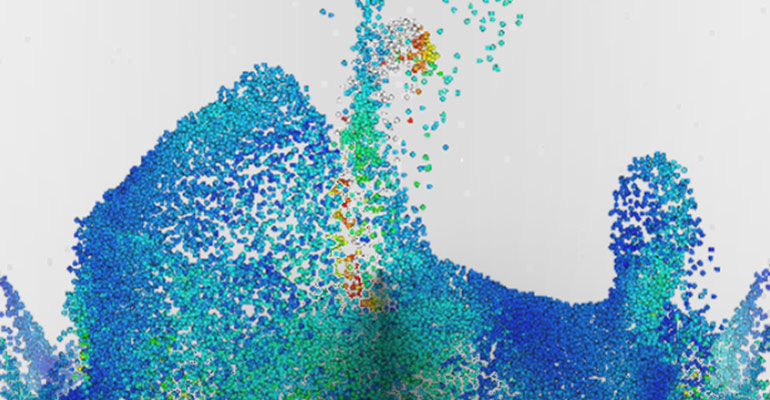
\includegraphics[width = 0.6\linewidth]{img/DEM}
  \end{figure}

 \end{itemize}
\end{frame}

\begin{frame}{Common-Plane}
 \begin{itemize}
  \item En 1988 Cundall\cite{1988-Cundall} propuso un algoritmo llamado Common-Plane (CP)
  \item Mencionando algunos algoritmos utilizados a lo largo de la historia son: CP, FCP, MR, SLM, Multi-grid y MSC entre otros.
  \item Estos algoritmos empezaron desde la misma base que ocupa el algoritmo Common-Plane.
 \end{itemize}
\end{frame}

\begin{frame}{Common-Plane}
 \begin{itemize}
  \item Common-Plane(CP), fue en primera instancia creado por Cundall en 1988.
  \item El principio de este algoritmo, es localizar un plano entre dos figuras e ir calculando la distancias.
  \begin{figure}[\centering]
  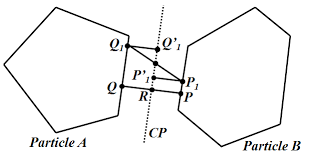
\includegraphics[width=0.5\linewidth]{img/CP}
  \end{figure}

 \end{itemize}
\end{frame}

\begin{frame}{Fast Common-Plane}
 \begin{itemize}
  \item En 2004 Nezami \cite{2004-Nezami} propuso una nueva propuesta para el calculo del CP y se llamo Fast Common-Plane (FCP).
  \item Con esta nueva propuesta mejoro el orden del algoritmo por ello la eficiencia.
  \begin{figure}[\centering]
  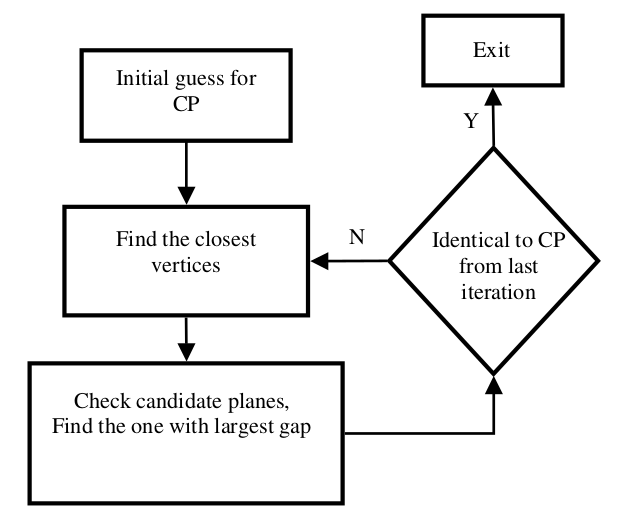
\includegraphics[width = 0.5\linewidth]{img/Diagrama-FCP}
  \end{figure}

 \end{itemize}
\end{frame}

\begin{frame}{Shortest Link Method}
 \begin{itemize}
  \item Nezami en 2006 \cite{2006-Nezami} propuso otro algoritmo el cual ocupa como base FCP.
  \item En base a resultados expuestos por Nezami \cite{2006-Nezami} SLM es 17 veces mas rápido que otros algoritmos convencionales.
  \begin{figure}[\centering]
  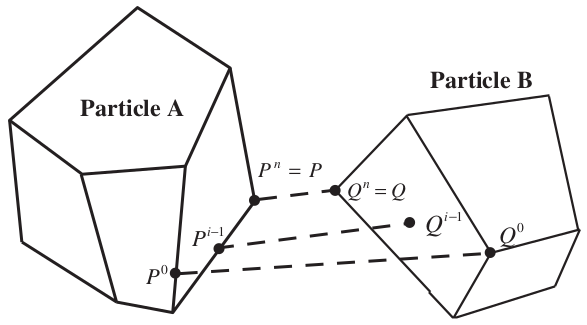
\includegraphics[width=0.5\linewidth]{img/SLM}
  \end{figure}
 \end{itemize}
\end{frame}

\begin{frame}{Multi-shell Contact Detection}
 \begin{itemize}
  \item Fue desarrollado por Zhuang el 2014 \cite{2014-Zhuang}.
  \item La detección de contacto y la búsqueda de vecindario.
  \item MSC como método tanto de detección de vecindario como detección de contacto es uno de los mas eficiente, según concluye Zhuang.
  \begin{figure}[\centering]
   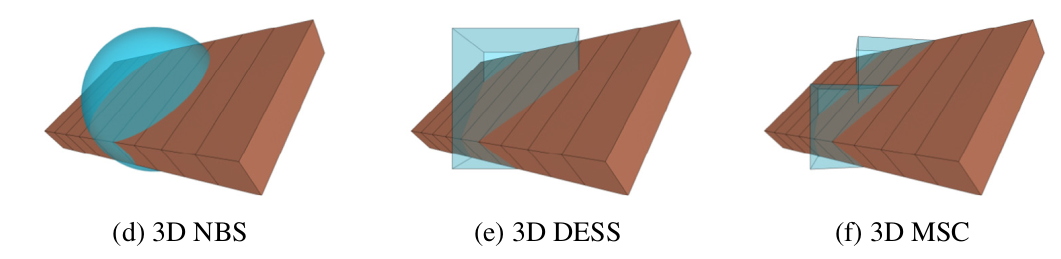
\includegraphics[width=0.8\linewidth]{img/Multi-shell}
  \end{figure}
 \end{itemize}
\end{frame}

\section{Problema}
\begin{frame}{Problema}
    \begin{itemize}
        \item Detección de contacto computacionalmente costoso.
        \item Análisis de gran cantidad de partículas.
    \end{itemize}
\end{frame}

\section{Objetivo}
\begin{frame}{Objetivo}

\begin{block}{Objetivo General}
 \begin{itemize}
    \item Detectar de forma eficiente y eficaz el contacto entre poliedros.
 \end{itemize}
\end{block}

\begin{block}{Objetivo Especifico}
 \begin{itemize}
  \item Generar algoritmo de detección de contacto mediante método propuesto.
 \end{itemize}
\end{block}
\end{frame}     

\section{Metodología}
\begin{frame}{Metodología}
\begin{itemize}
    \item Se realizo un estudio sobre el tema propuesto, donde se recopilaron los datos pertinentes.
    \item Se genero una linea de tiempo donde se señalaron los trabajos mas relevantes al tema.
\end{itemize}
\end{frame}

\begin{frame}{Metodología}
\begin{itemize}
    \item Principales framework de trabajo son github, pycharm, kile y overleaf.
\end{itemize}
    \begin{figure}
     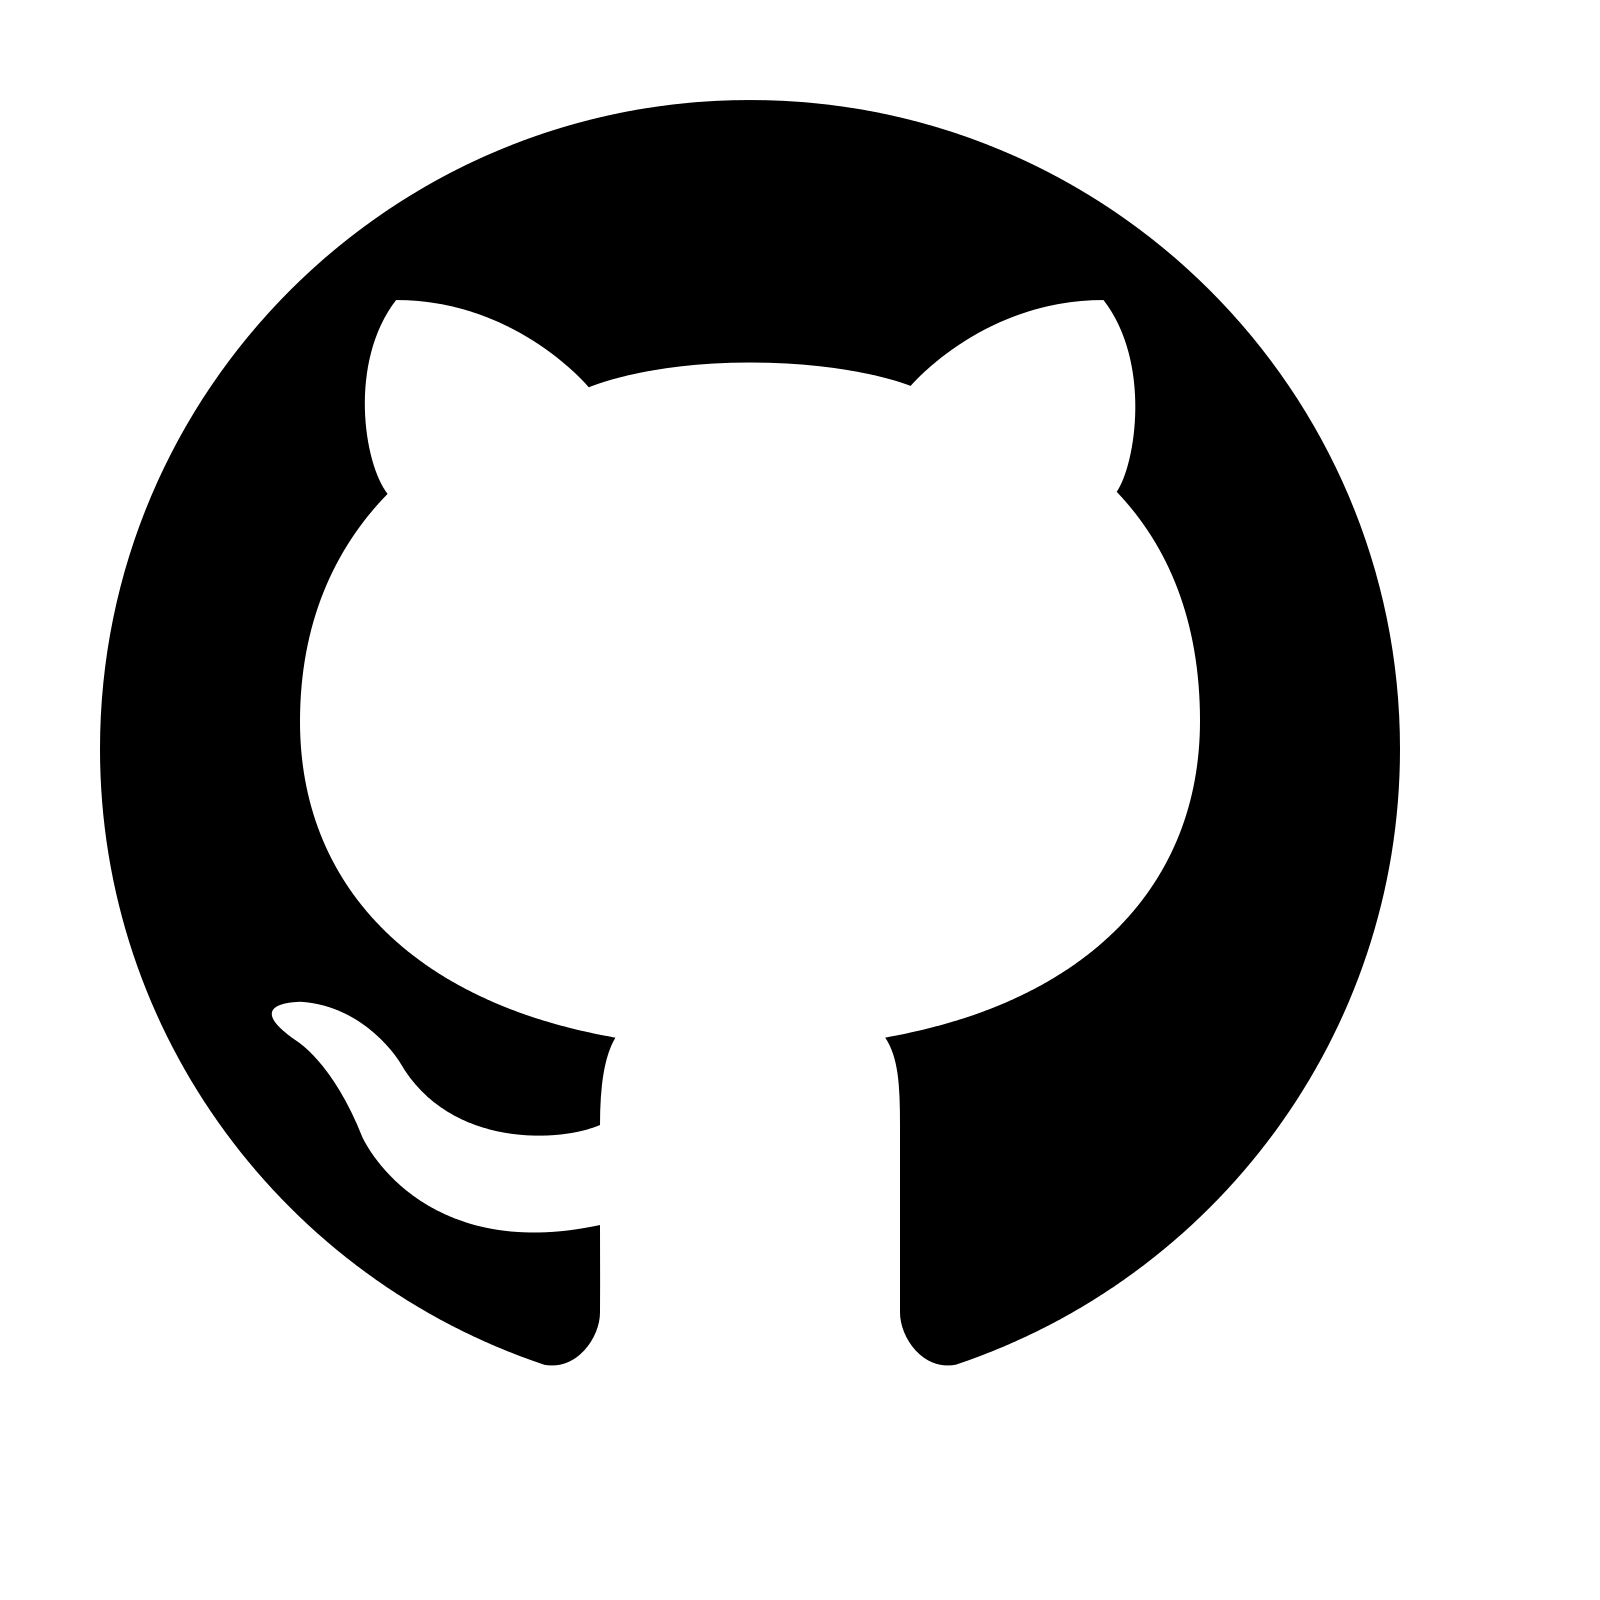
\includegraphics[width = 0.2\linewidth]{img/github_logo}
     
\includegraphics[width = 0.2\linewidth]{img/pycharm}
     
\includegraphics[width = 0.2\linewidth]{img/kile}
     
\includegraphics[width = 0.2\linewidth]{img/Overleaf}
    \end{figure}
\end{frame}

\begin{frame}{Metodología}
 \begin{block}{Algoritmo}
\begin{figure}
 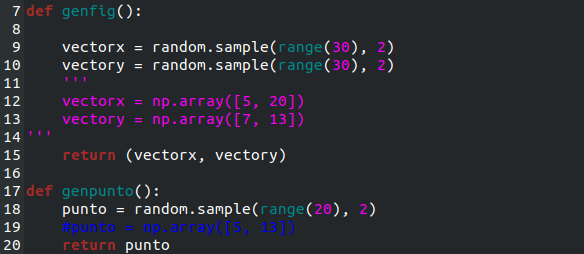
\includegraphics[width = 0.6\linewidth]{img/figure_gen}
\end{figure}
 \end{block}
\end{frame}

\begin{frame}{Metodología}
 \begin{block}{Algoritmo}
\begin{figure}
 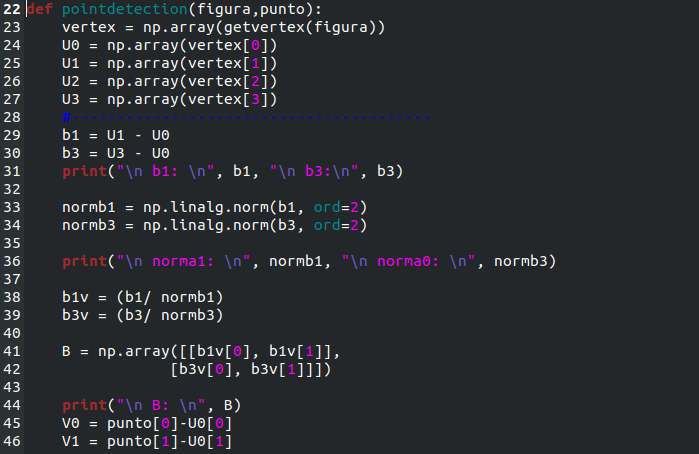
\includegraphics[width = 0.6\linewidth]{img/Contact_detection}
 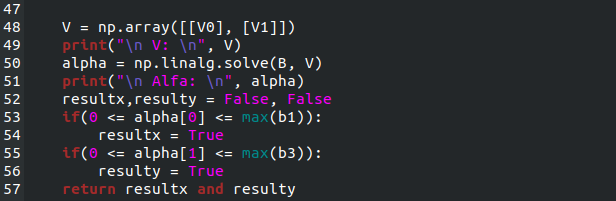
\includegraphics[width = 0.6\linewidth]{img/Contact_detection2}
\end{figure}
 \end{block}
\end{frame}

\begin{frame}{Metodología}
 \begin{block}{Algoritmo}
\begin{figure}
 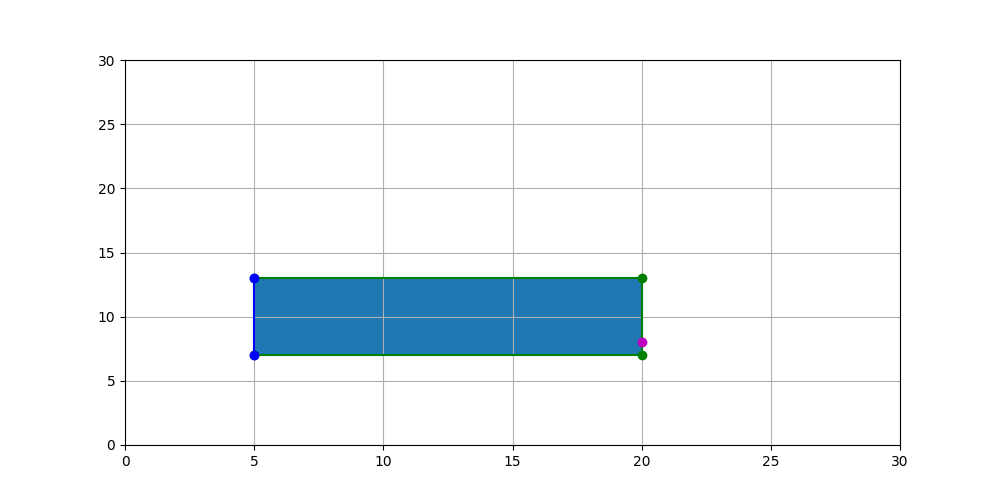
\includegraphics[width = 0.6\linewidth]{img/Figura_arista}
 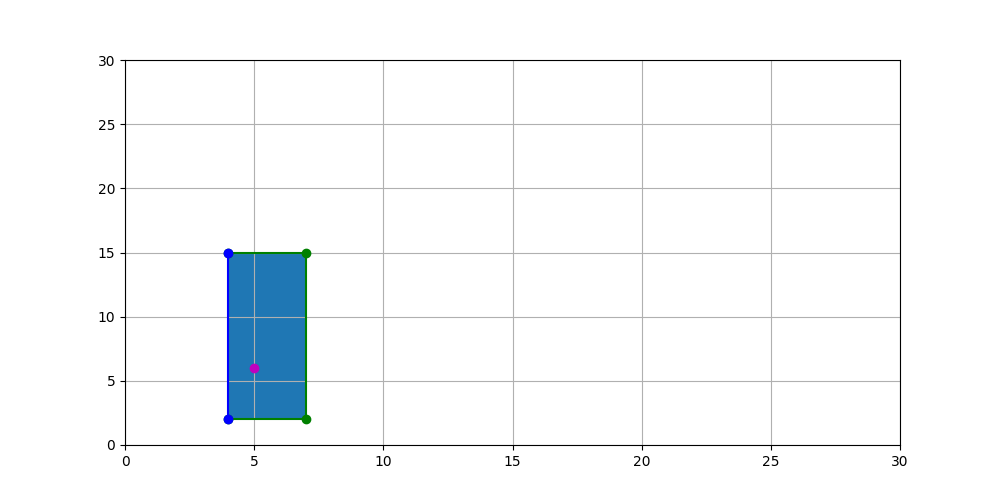
\includegraphics[width = 0.6\linewidth]{img/Figura_dentro}
\end{figure}
 \end{block}
\end{frame}

\begin{frame}{Metodología}
 \begin{block}{Algoritmo}
\begin{figure}
 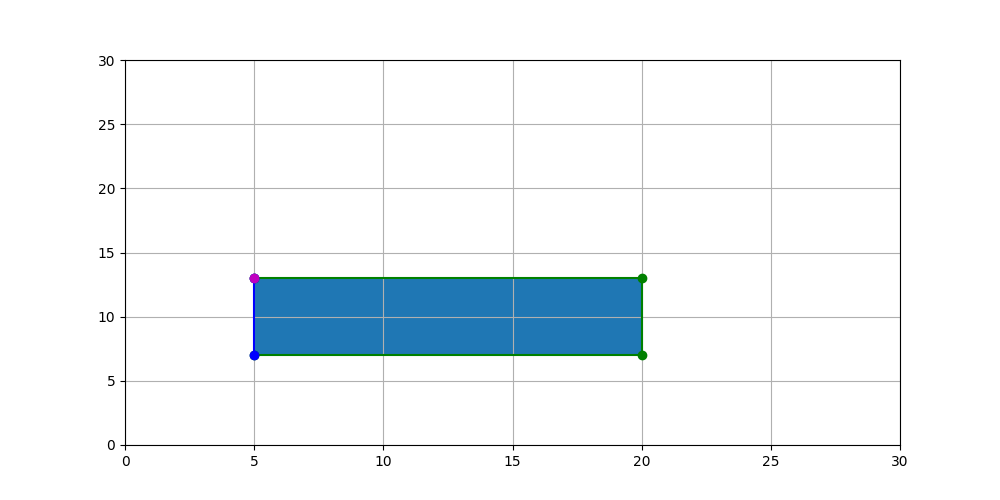
\includegraphics[width = 0.6\linewidth]{img/Figura_vertice}
 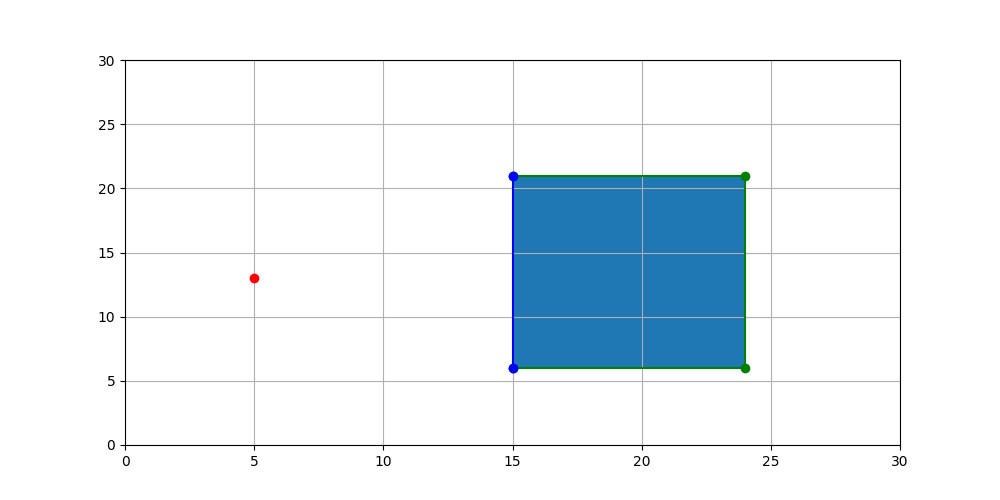
\includegraphics[width = 0.6\linewidth]{img/figura_fuera}
\end{figure}
 \end{block}
\end{frame}

\begin{frame}{Metodología}
\begin{itemize}
    \item Para el control de versiones del código se utilizo un repositorio en github.
    \begin{figure}
      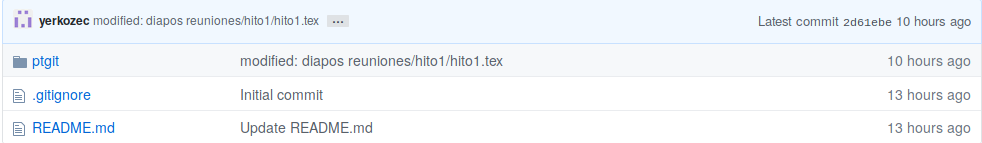
\includegraphics[width = 1\linewidth]{img/github}
    \end{figure}

\end{itemize}
\end{frame}

\section{Conclusion}
\begin{frame}{Conclusion}
 \begin{itemize}
  \item Cabe mencionar que existen varias soluciones al problema propuesto, pero aun así no esta completamente resuelto.
  \item Se busca realizar la detección de contacto de la forma más eficiente posible ocupando la menor cantidad de recursos computacionales posibles.
 \end{itemize}
\end{frame}

\section{Referencias}
\begin{frame}{Referencias}
\medskip
\bibliographystyle{plain}
\bibliography{/home/yerkozec/Desktop/pt/memoria/Referencia}
\end{frame}


\begin{frame}[plain]
  \titlepage
\end{frame}

\end{document}
